\chapter{Análisis comparativo}
Android e iOS son dos plataformas muy populares entre los dispositivos móviles. Es por ello, que existes muchas  muchas formas de comparar sus respectivos módulos de seguridad.\\
La medida de comparación propuesta en \cite{YA2014} consiste en analizar la seguridad de una aplicación móvil en cada fase del ciclo de vida, comparándola en cada plataforma.\\
En \cite{HYGZD2013} el enfoque es distinto. Se centra en comparar los permisos requeridos a cada plataforma al momento de instalar aplicaciones presentes en ambas plataformas.\\
En \cite{Gor16, BCLR15, Rom14} se cambia el enfoque propuesto. El objetivo que persiguen es desarrollar una especificación formal que describa el modulo de seguridad de Android.\\
En este capítulo se propone una forma de comparar distinta a las anteriores. Consiste en analizar distintas características presentes en ambas plataformas, poniendo foco especialmente en los permisos que se pueden modificar en tiempo de ejecución. El análisis se esta basado en los documentos oficiales de seguridad, tales como \cite{aossec, asreview2015, asg} entre otros. Al final del capítulo se agrega una crítica sobre las funcionalidades mencionadas en el análisis.\\
\section{Analizando Android}
\subsection{Seguro desde el arranque}
Android ofrece la funcionalidad de garantizar un arranque seguro del dispositivo, comenzando desde un lugar confiable del \textit{hardware} hasta que se monta la partición. Durante el arranque, el sistema operativo verifica que la versión de Android no se haya alterado respecto a la de fábrica, informando mediante alertas en caso contrario y ofreciendo opciones para resolverlo. Dependiendo de la implementación de la funcionalidad, el sistema operativo puede ofrecer una acción al usuario o evitar el arranque hasta que se haya solucionado el problema \cite{aossec}.\\
En la figura \ref{fig:ch03:verifyBoot} se observa el diagrama de flujo del \textit{Arranque Seguro\footnote{Traducción del término \textit{Verified Boot}.}}, el cual termina en cuatro estados posibles:
\begin{itemize}
	\item Verde: indica que se pudo verificar correctamente el arranque del sistema.
	\item Amarillo: indica que se pudo validar el certificado correspondiente a la partición de arranque. Requiere la huella dactilar para continuar el inicio.
	\item Naranja: indica que el dispositivo pudo ser modificado, ya que no se pudo verificar la partición de arranque. Requiere acción del usuario para continuar.
	\item Rojo: indica que falló la verificación. Es decir, no pudo validar ninguna partición.
\end{itemize}
\begin{figure}[hbtp]
	\begin{center}
		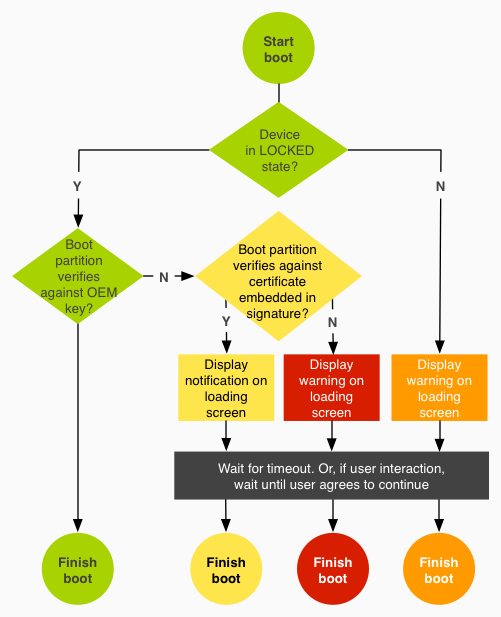
\includegraphics[width=0.6\linewidth]{chapter3/verified_boot}
		\caption{Diagrama de flujo del \textit{Arranque seguro} \cite{asreview2015}.}
		\label{fig:ch03:verifyBoot}
	\end{center}
\end{figure}
\subsection{Cifrado de la partición de datos}
Mediante una opción de la configuración, Android permite cifrar todos los datos de usuario presentes en un dispositivo, utilizando claves de cifrado simétricas. Una vez cifrado, el proceso es transparente para el usuario. Es decir, todos los datos creados se cifran antes de enviarlos al disco y todas las lecturas descifran los datos antes de devolverlos al proceso que realizó la llamada.\\
Esta funcionalidad se activa desde \texttt{Ajustes/Seguridad/Cifrar Teléfono}, como se observa en la Figura \ref{fig:ch03:android-cifrado}. Al activarse dicha opción, se cifran los datos privados de las aplicaciones, el contenido de la tarjeta SD y los datos personales, pudiendo cambiar más adelante el alcance de los componentes afectados por el cifrado. Mientras esté activa dicha opción, cada vez que arranque el dispositivo, el usuario debe proporcionar sus credenciales para poder acceder a cualquier parte del disco.\\
La primera vez que apareció esta funcionalidad fue en la versión 3.0. Sin embargo, a partir de la versión 5.0, fue fuertemente recomendado a los fabricantes de dispositivos que habiliten esta característica. La novedad incorporada en Android Marshmallow es que se puede cifrar el contenido de la tarjeta SD, permitiendo que sea ilegible si es removida del dispositivo.\\
\begin{figure}[hbtp]
	\begin{center}
		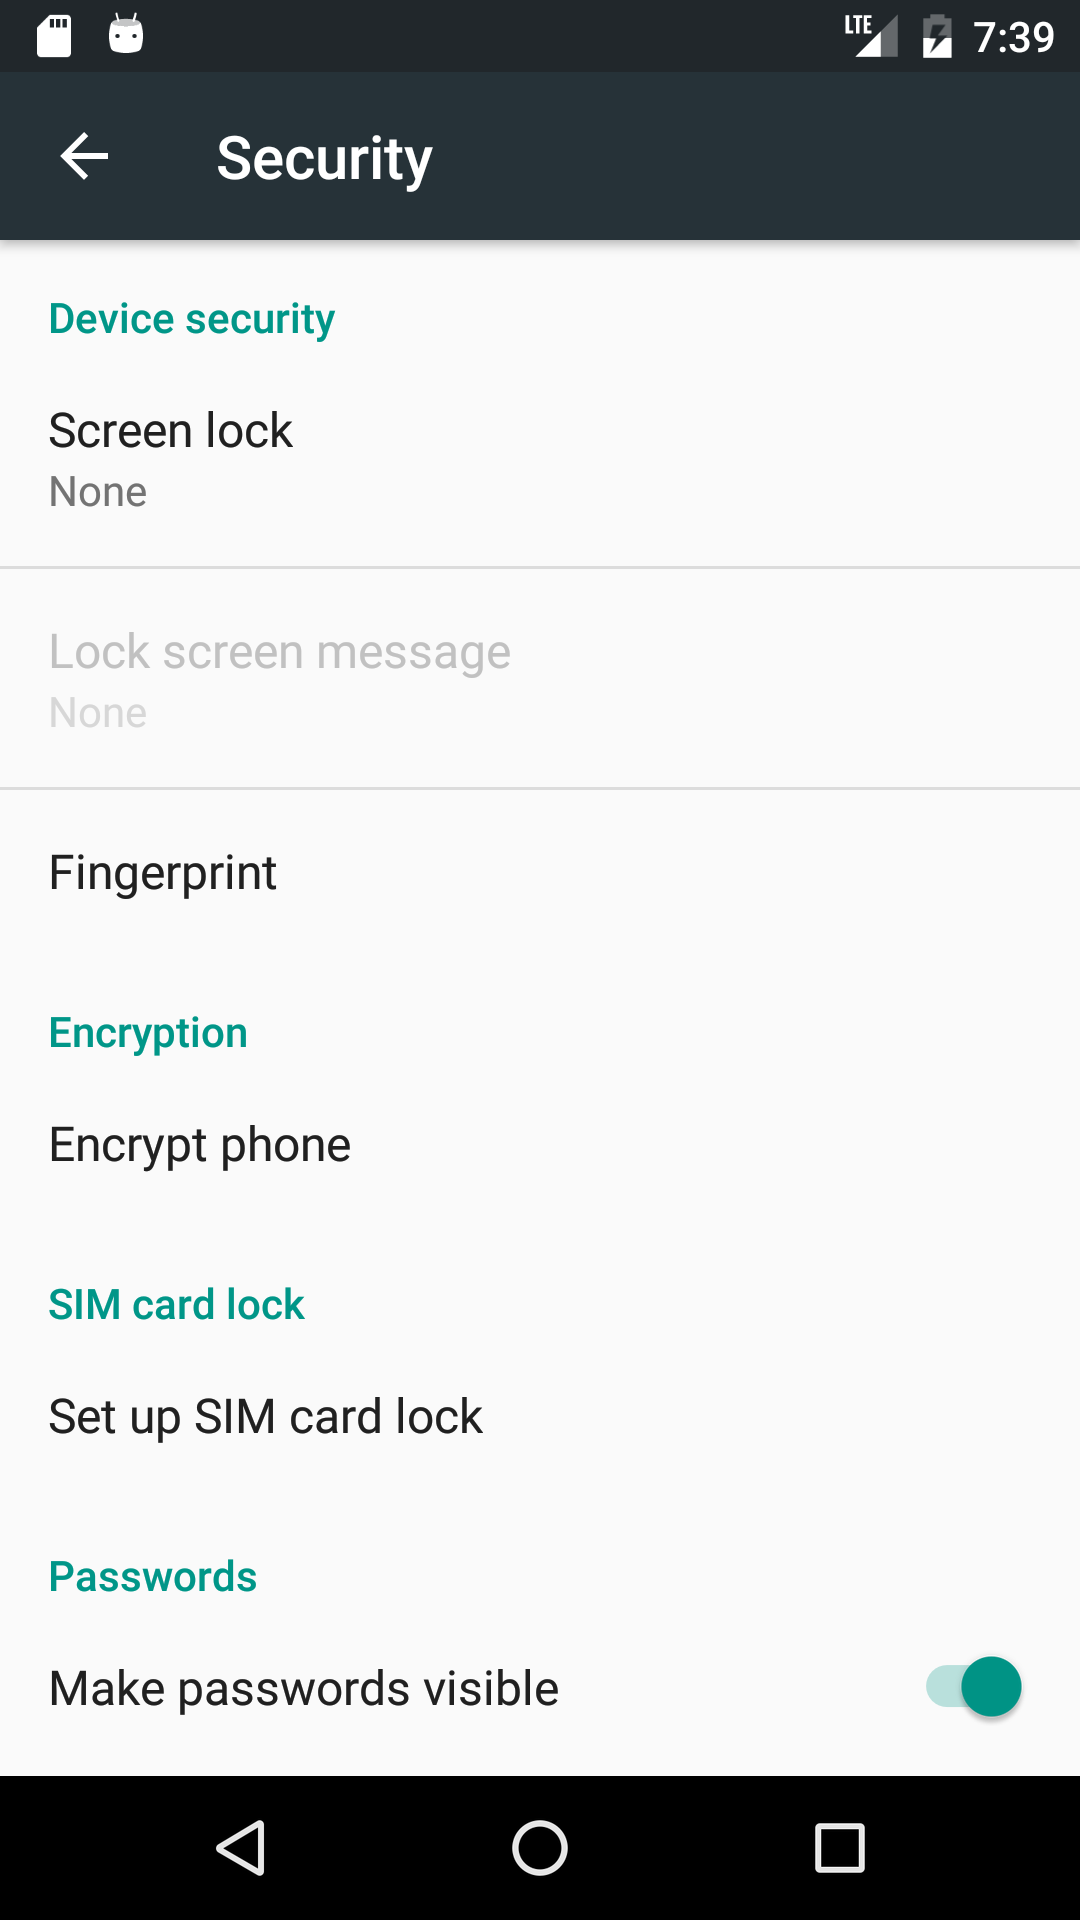
\includegraphics[width=0.3\linewidth]{chapter3/android-cifrado}
		\caption{Captura de \texttt{Ajustes/Seguridad}.}
		\label{fig:ch03:android-cifrado}
	\end{center}
\end{figure}
\subsection{Permisos}
Debido a que cada aplicación Android opera en un entorno aislado\footnote{Ver seccion \nameref{ch01-sandbox}.}, las aplicaciones deben compartir de manera explícita recursos y datos. El camino utilizado para realizar dicho intercambio es la declaración de permisos, tal como se introdujo en la sección \ref{ch01-permisos}. El presente informe se centra en los permisos \emph{Normal} y \emph{Dangerous}; cómo se otorgan y cómo se deniegan.\\
En las versiones anteriores a Android Marshmallow, al prepararse para instalar una aplicación, el sistema operativo mostraba un diálogo al usuario indicando los permisos solicitados y se le solicitaba si deseaba continuar con la instalación. En caso afirmativo, el sistema otorgaba todos los permisos solicitados e instalaba la aplicación. En el caso contrario, no se instalaba la aplicación. El usuario quedaba preso si quería instalar una aplicación: no podía otorgar o denegar permisos individuales; debía otorgar o denegar todos los permisos solicitados como un bloque. Una vez concedidos, los permisos seguían vigentes mientras la aplicación este instalada. Solo se eliminaban si se desinstala dicha aplicación.\\
\begin{figure}[hbtp]
    \centering
        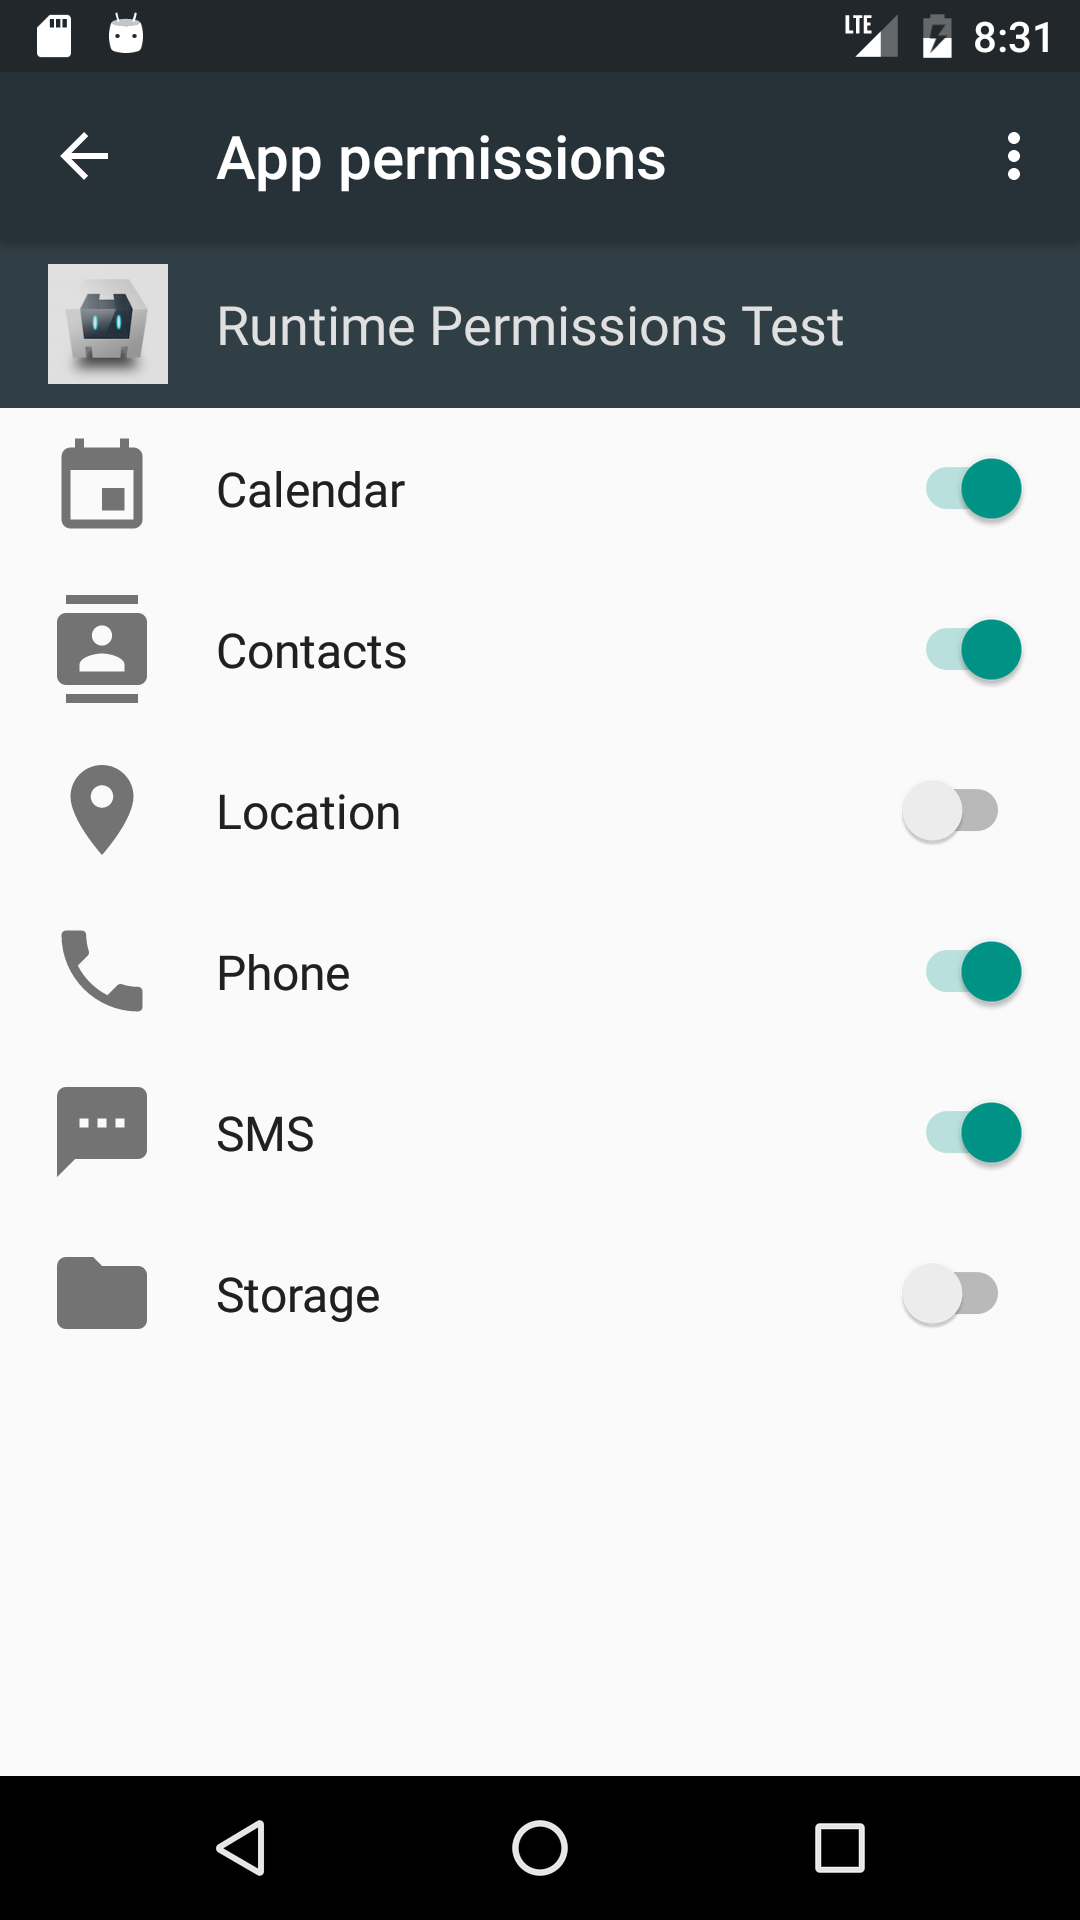
\includegraphics[width=.3\linewidth]{imgs/chapter1/app-permissions}
    \caption{Descripción general de los permisos otorgados.}
	\label{fig:ch01:app-permissions-overview}
\end{figure}
A partir de la versión 6.0, se propone un nuevo modelo de permisos, donde los usuarios pueden administrar en tiempo de ejecución los permisos \textit{peligrosos} requeridos por una aplicación. En este modelo, los permisos se agrupan para facilitar el control de la privacidad de los usuarios. Dichos grupos son:
\begin{itemize}
    \item \emph{Almacenamiento:} Regula el acceso al almacenamiento externo\footnote{En Android, cuando se habla de almacenamiento externo, se refiere a la tarjeta SD.}, \\permitiendo la lectura o la escritura desde el mismo.
    \item \emph{Calendario:} Permite leer, modificar o eliminar los calendarios del usuario. Incluye además el manejo de los eventos presentes en un calendario.
    \item \emph{Cámara:} Regula el acceso de la cámara del dispositivo, permitiendo capturar imágenes y grabar videos.
    \item \emph{Contactos:} Permite leer, modificar o eliminar los contactos presentes en el dispositivo.
    \item \emph{Localización:} Regula el acceso a la ubicación del dispositivo, ya sea la ubicación precisa (GPS) o la ubicación aproximada (WIFI/Móvil).
    \item \emph{Mensajes SMS:} Permite escribir mensajes SMS, leerlos o eliminarlos. Además, permite interceptar los mensajes entrantes.
    \item \emph{Micrófono:} Regula el acceso al micrófono del dispositivo, permitiendo además grabar el sonido obtenido. No se incluyen en este grupo los permisos para capturar sonidos provenientes de una llamada telefónica.
    \item \emph{Teléfono:} Regula el acceso a la información relacionada a una llamada telefónica, tales como iniciar una llamada, obtener datos de una llamada en curso, manipular el log de llamadas, entre otros.
    \item \emph{Sensores:} Permite acceder a los datos de los sensores del dispositivo. Se incluyen el giroscopio, el acelerómentro, sensor del ritmo cardíaco, entre otros.
\end{itemize}
En contraposición a lo que ocurría en las versiones previas, en Android Marsmallow durante la instalación de una aplicación no se concede ningún permiso \textit{peligroso}. Cada vez que una aplicación necesita acceder a un recurso protegido por un permiso \textit{peligroso}, tiene que solicitarlo en tiempo de ejecución. Por ejemplo, si una aplicación requiere leer un contacto, la primera vez aparece una notificación pidiendo autorización explicita al usuario, tal como se observa en la Figura \ref{fig:ch01:permission-request}. El usuario puede otorgar el permiso, denegarlo una vez o denegarlo para siempre. Si elige la última opción, no volverá a aparecer la notificación solicitando dicho permiso. De querer otorgar el permiso, el usuario va a tener que realizarlo manualmente desde \texttt{Ajustes/Aplicaciones/\{nombre de la aplicación\}/Permisos}. Ya que el usuario puede revocar los permisos en cualquier momento, una aplicación debe comprobar si dispone de los permisos cada vez que se ejecuta. De lo contrario no va a poder acceder a las funciones de las cuales no tiene permiso.
\begin{figure}[htbp]
    \centering
    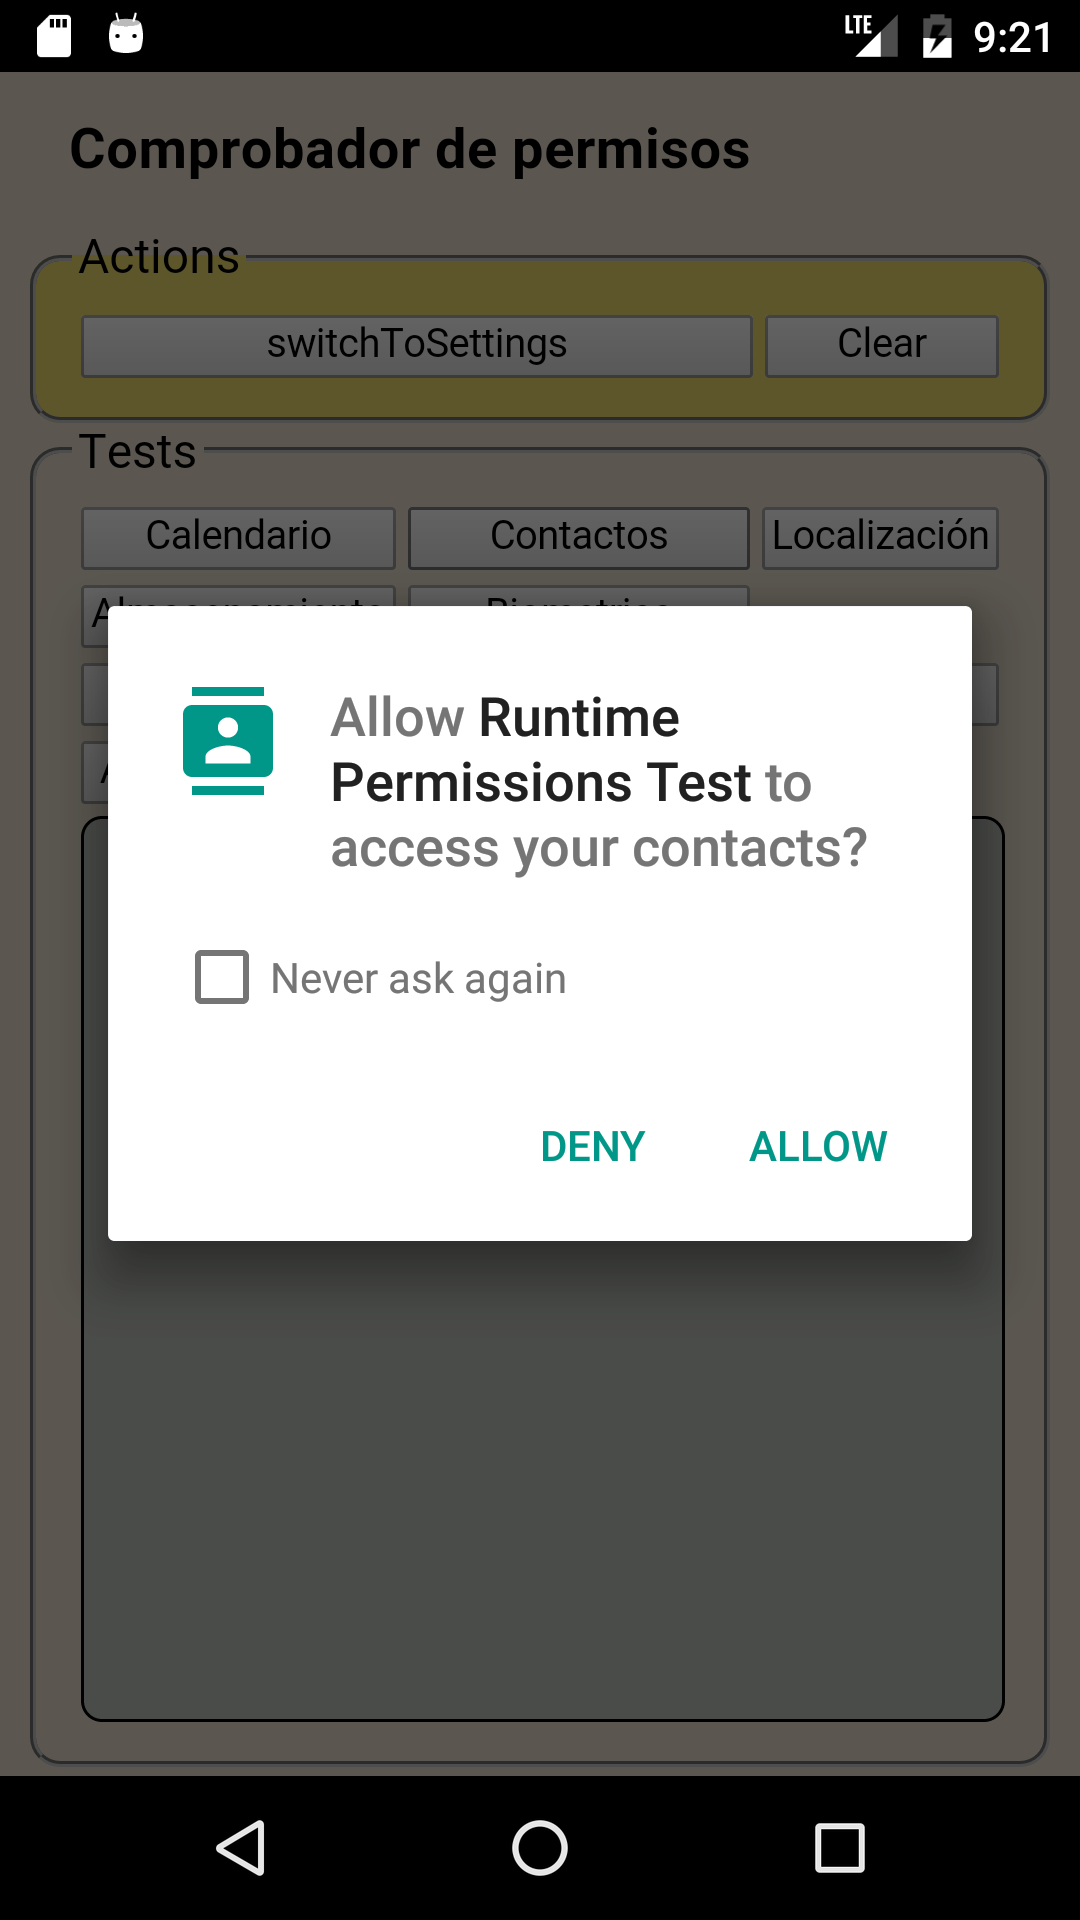
\includegraphics[width=0.3\linewidth]{imgs/chapter5/allow_contact}
    \caption{Ejemplo de solicitud de un permiso en tiempo de ejecución.}
    \label{fig:ch01:permission-request}
\end{figure}
\section{Analizando iOS}
\subsection{Arranque seguro}\label{fig:ch02:arranque}
Cada dispositivo es seguro desde el arranque \cite{asg}, ya que la arquitectura del sistema fue pensada para integrar \textit{software} y \textit{hardware} de manera tal que de asegurar que cada componente sea seguro. Cuando se prende un dispositivo cuyo sistema operativo es iOS, se siguen los siguientes pasos para asegurar la integridad del arranque del sistema (\textit{Boot Chain}):
\begin{enumerate}
	\item Se ejecuta el código alojado en la \textit{BootROM}. Es inmutable y seguro por definición.
	\item Se verifica la firma del \textit{bootloader} LLB (\textit{Low Level Bootloader}, por sus siglas en ingl\'es), ya que fue certificado por Apple con la clave pública \textit{Apple Root CA}. La misma está alojada en la \textit{BootROM}. 
	\item Pasada la validación, empieza la carga del kernel de iOS mediante \textit{iBoot}.
	\item El siguiente paso es asegurar la integridad del software. Los dispositivos con un procesador A7 o superior, cuentan con un co-procesador llamado \textit{Secure Enclave \footnote{\textit{Secure Enclave} es un co-procesador con memoria encriptada e incluye generación de números aleatorios por hardware \cite{asg}.}} para verificar dicha integridad.
\end{enumerate}
Si fallan alguno de estos pasos, el dispositivo entra en Modo de Recuperación (\textit{recovery mode}) y se lo debe conectar a iTunes via USB para restaurar la configuración de fábrica.\\
Nos detendremos en el componente llamado \textit{Secure Enclave}. Tiene dos funciones principales \cite{asg}: proveer todas la operaciones criptográficas para la manipulación de la clave de los datos (\textit{Data Protection Key}); y mantener la integridad de dichos datos inclusive si se haya violado la seguridad del \textit{kernel}.\\
Dentro de las claves que almacena, se encuentra la clave única UID\footnote{\textit{Unique ID}, por sus siglas en inglés}, que fue creada en el momento de fabricación y que no es conocida por Apple ni por ningún otro componente del dispositivo. La misma es utilizada para generar una clave efímera cada vez que se prende el dispositivo, la cual se utiliza para encriptar la memoria del \textit{Secure Enclave} y para encriptar los datos del sistema de archivos.\\
Por último, el \textit{Secure Enclave}, se encarga también de procesar los datos que llegan desde el lector de huellas (\textit{Touch ID}), determinando si se puede desbloquear el dispositivo.
\subsection{Permisos}
Los controles de privacidad en iOS dan el control sobre qué aplicaciones tienen acceso a la información almacenada en su dispositivo iOS. Su enfoque es distinto ya que focaliza en componentes del sistema, permitiendo al usuario denegar (o permitir) el acceso de una aplicación a un determinado componente. El usuario puede modificar la configuración de privacidad en $Ajustes > Privacidad$. En ella se encuentra una lista de componentes, como se observa en la figura \ref{fig:chapter03:iospermCapture}. Para cada uno de ellos, figuran las aplicaciones que pidieron permiso para usar dicho componente. Se pueden agregar o quitar el permiso de cualquier aplicación que ha solicitado el acceso a los datos. Cabe aclarar que una aplicación puede utilizar sus datos sólo si se le ha dado permiso.\\

\begin{figure}[!pb]
	\begin{subfigure}{.4\textwidth}
		\centering
		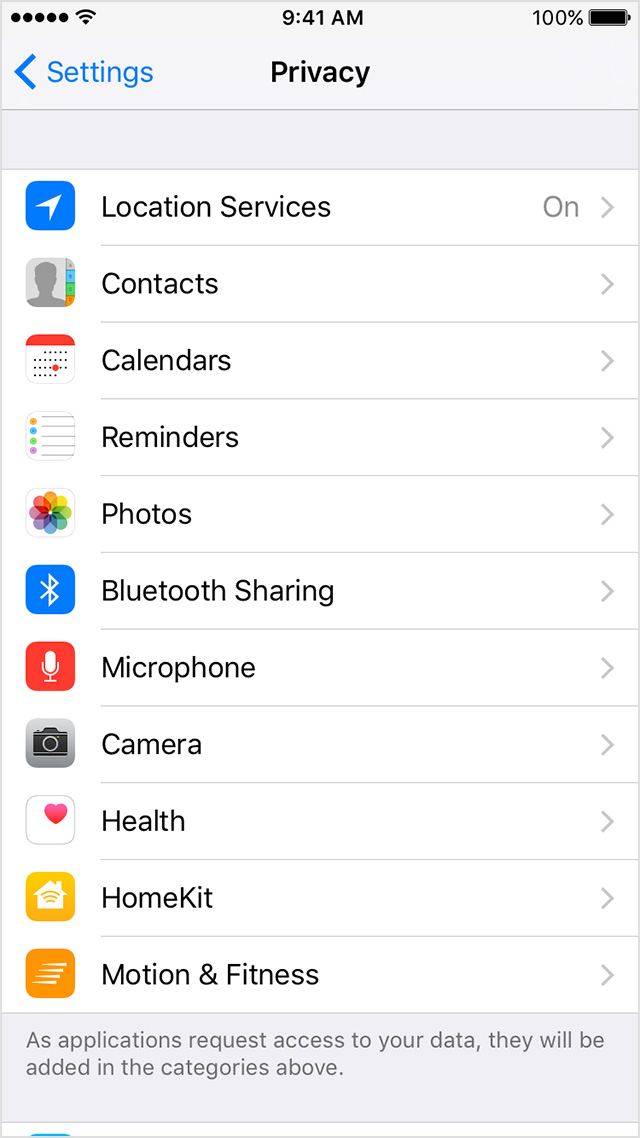
\includegraphics[width=135px]{chapter3/iphone6-ios9-settings-privacy}
    		\caption{iOS 9.3}
   		\label{fig:chapter03:iospermCapture}
	\end{subfigure}
	\begin{subfigure}{.55\textwidth}
	    \centering	
		\begin{tabular}{|c|c|}
			\hline
			Permissions		 					& Subgroup\\ \hline
			\multirow{12}{*}{LOCATION SERVICES} 	& Cell Network Search \\
								 				& Compass Calibration \\
												& Find My iPhone \\
												& HomeKit \\
												& Location-Based Alerts \\
												& Location-Based iAds \\
												& Motion Calibration \& Distance \\
												& Safari \& Spotlight Suggestions \\
												& Settings Time Zone\\
												& Share My Location \\
												& Wi-Fi Networking \\
												& Frequent Locations \\ \hline
			Contacts				& \\ \hline
			Calendars			& \\ \hline
			Reminders			& \\ \hline
			Photos				& \\ \hline
			Bluetooth Sharing 	& \\ \hline
			Microphone 			& \\ \hline
			Camera 				& \\ \hline
			Health 				& \\ \hline
			HomeKit 				& \\ \hline
			Social Media Accounts& \\ \hline
			Diagnostics \& Usage	& \\ \hline		
			Advertising			& \\ \hline
		\end{tabular}
		\caption{Permisos modificables por el Administrador de Privacidad de iOS}
		\label{tab:chapter03:iosperm}
	\end{subfigure}
\end{figure}
La lista mencionada anteriormente contiene algunos componentes cuyo nombre es lo suficientemente descriptivo como para saber que estamos permitiendo o denegando. A continuación se hará una breve descripción sobre los componentes de la lista:
\begin{itemize}
	\item \textbf{Location Services:} permite a las aplicaciones y/o a las páginas web determinar aproximadamente su ubicación. Dependiendo de su dispositivo y de los servicios disponibles, se utiliza una combinación de cierta información del celular, Wi-Fi, Bluetooth y GPS para determinar su ubicación.
	\item \textbf{Contacts:} permite a las aplicaciones el acceso a los contactos.
	\item \textbf{Calendars:} regula el acceso a los calendarios, incluyendo las citas y eventos incluidos en él.
	\item \textbf{Reminders:} permite a las aplicaciones la lectura y/o escritura de los recordatorios.
	\item \textbf{Photos:} permite a una aplicación el acceso a las fotos y al álbum de cámara directamente, ya sea para subir nuevas imágenes a un servicio desde el dispositivo iOS, o para guardar nuevas imágenes a la aplicación Fotos. También pueden tener la capacidad de crear un álbum de fotos dentro de la aplicación de fotos.
	\item \textbf{Bluetooth Sharing:} permite controlar cuáles aplicaciones pueden compartir datos a través de Bluetooth.
	\item \textbf{Microphone:} regula el acceso al micrófono.
	\item \textbf{Camera:} regula el acceso al la cámara del dispositivo.
	\item \textbf{Health:} permite a las aplicaciones conocer la información de su salud y estado físico, tanto las cargadas como las que recopiló el dispositivo.
	\item \textbf{HomeKit:} regula el acceso a los accesorios hogareños registrados en el dispositivo.			
	\item \textbf{Social Media Accounts:} permite a las aplicaciones realizar actividades relacionadas a una red social, tales como crear una sesión de red, obtener el feed de actividad para un usuario, hacer una nueva entrada. También permite publicar una entrada a un canal de actividades o realizar ajustes de las propiedades de una publicación, añadir archivos adjuntos, etc.
	\item \textbf{Diagnostics \& Usage:} regula cuáles datos de diagnóstico sobre el dispositivo se envían a Apple. Esos datos incluyen información sobre el rendimiento del sistema, capacidad restante en el dispositivo, detalles acerca de sus especificaciones del dispositivo y del sistema operativo, entre otras.
	\item \textbf{Advertising:} permite inhabilitar los anuncios basados en intereses.
\end{itemize}
\newpage

\section{Crítica}
Al momento de realizar el análisis, se tuvieron en cuenta las coincidencias y las diferencias entre ambas plataformas.\\
Entre las primeras, podemos mencionar que las dos tienen dispositivos en común a los cuáles se les pueden modificar permisos en \textit{runtime}: micrófono, cámara, GPS, y sensores biométricos. También se aplican dichos permisos a componentes que contienen información sensible del usuario, tales como el calendario, los contactos y las fotos.\\
Entre las segundas, podemos mencionar permisos que tiene uno pero no el otro. Por ejemplo, Android tiene la permisos sobre el almacenamiento externo. Este permiso no tiene sentido en iOS, ya que los iPhone solamente tienen almacenamiento interno. iOS, por su parte, tiene integrado el manejo de ciertos dispositivos hogareños. También dispone de un servicio tracking de publicidad, el cual permite recomendaciones sobre los gustos del usuario. Por ello, agrega permisos para dichos componentes, los cuales no existes como componentes en Android.\\
Como consecuencia de lo mencionado anteriormente, se encontraron permisos que son comparables entre sí y otros que no lo son. Cabe aclarar que ciertos permisos se agruparon. Por ejemplo, en Android, los recordatorios forman parte del calendario; mientras que en iOS están separados. Los resultados se volcaron en la tabla \ref{tab:chapter03:compPerm}.\\

\begin{table}[!ht]
	\center
	\begin{tabular}{|c|c|c|}
		\hline
		\multicolumn{3}{|c|}{Permissions} \\					\hline
		Commons 	& Only Android	& Only iOS \\				\hline
		Calendar\&Events	& -		& -	\\						\hline
		Contacts	& -				& - \\						\hline
		Camera		& -				& -	\\						\hline
		Location	& -				& -	\\						\hline
		-			& -				& Bluetooth Sharing \\		\hline
		Microphone  & -				& - \\						\hline
		-			& Phone			& -	\\						\hline
		Body Sensors	& -			& - \\						\hline
		-			& SMS			& - \\						\hline
		-			& Storage		& - \\						\hline
		-			& -				& Homekit \\				\hline
		-			& -				& Social Media Accounts \\	\hline
		-			& -				& Diagnostic \& Usage \\	\hline		
		-			& -				& Advertising \\			\hline
	\end{tabular}
	\caption{Comparación de permisos entre Android 6.0 e iOS}
	\label{tab:chapter03:compPerm}
\end{table}
Para finalizar el capítulo, se mencionan las conclusiones que se encontraron.\\
Es importante destacar la falta de granularidad en algunos aspectos. Android no toma como permiso peligroso los datos de las redes sociales. Tampoco el permiso para compartir cosas por Bluetooth. Por otro lado, iOS no tiene la suficiente granularidad para administrar el acceso a las llamadas telefónicas, su historial, etc. Tampoco contempla los datos móviles ni los SMS. En estos casos, el permiso es a nivel de teléfono y no a nivel de aplicación.\\

Otra cosa a destacar es que en Android el permiso es a nivel de grupo. Cuando se requiere que el usuario permita cierto permiso para una aplicación, lo que sucede es que la aplicación obtiene todos los permisos del grupo. Por ejemplo, si se pide permisos del grupo "Calendario" se obtienen los permisos tanto para leer y para escribir. Para el caso del calendario puede llegar a ser razonable tener los dos permisos pero para otros casos no lo es. Como consecuencia de ello, el usuario esta delegando a una aplicación demasiados permisos.
\subsection*{Detalle de los tests}
Luego de instalar la aplicación, se observa que la misma no tiene ningún permiso:
\begin{figure}[!ht]
	\centering
	\begin{subfigure}{.32\textwidth}
		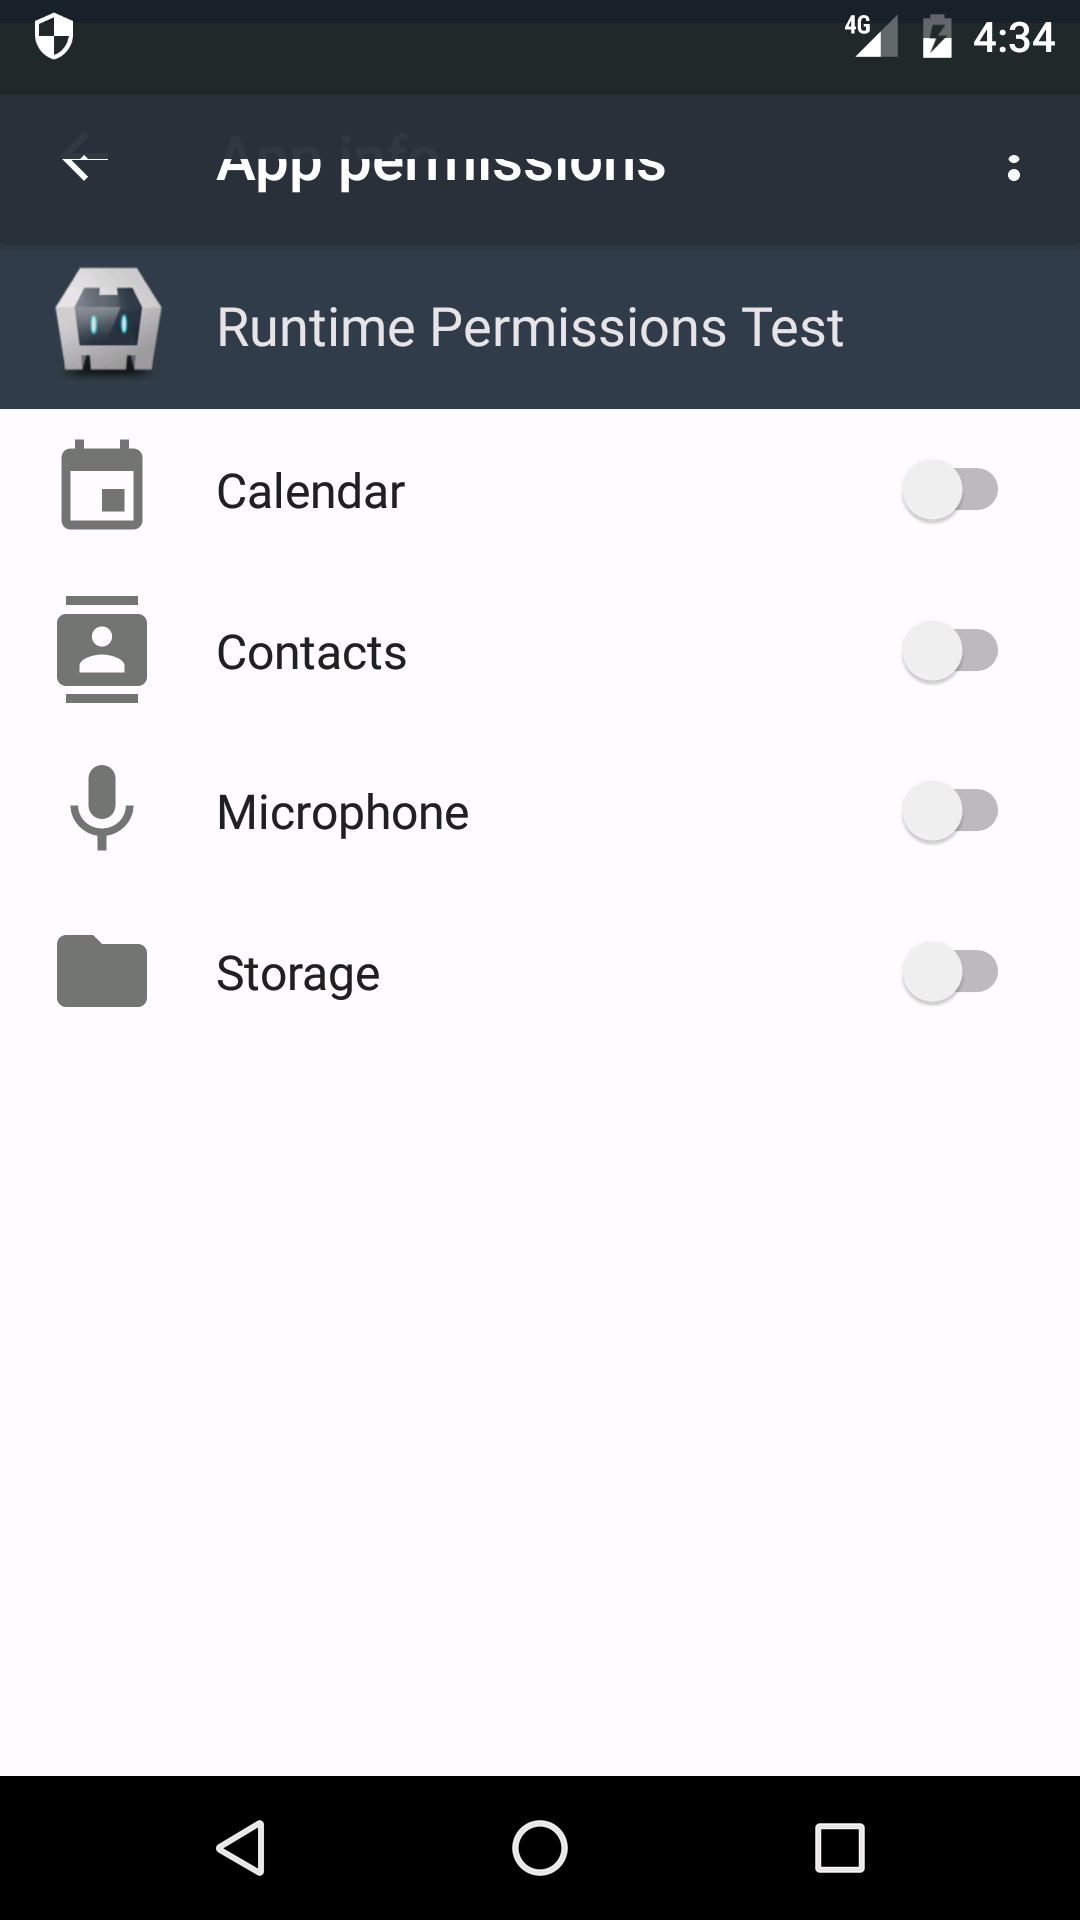
\includegraphics[width=4cm]{chapter5/without_permissions}
		\caption{\textit{Runtime Permissions Test} no tiene ningún permiso $peligroso$}
		\label{fig:chapter05:without_permissions}
	\end{subfigure}
	\begin{subfigure}{.32\textwidth}
		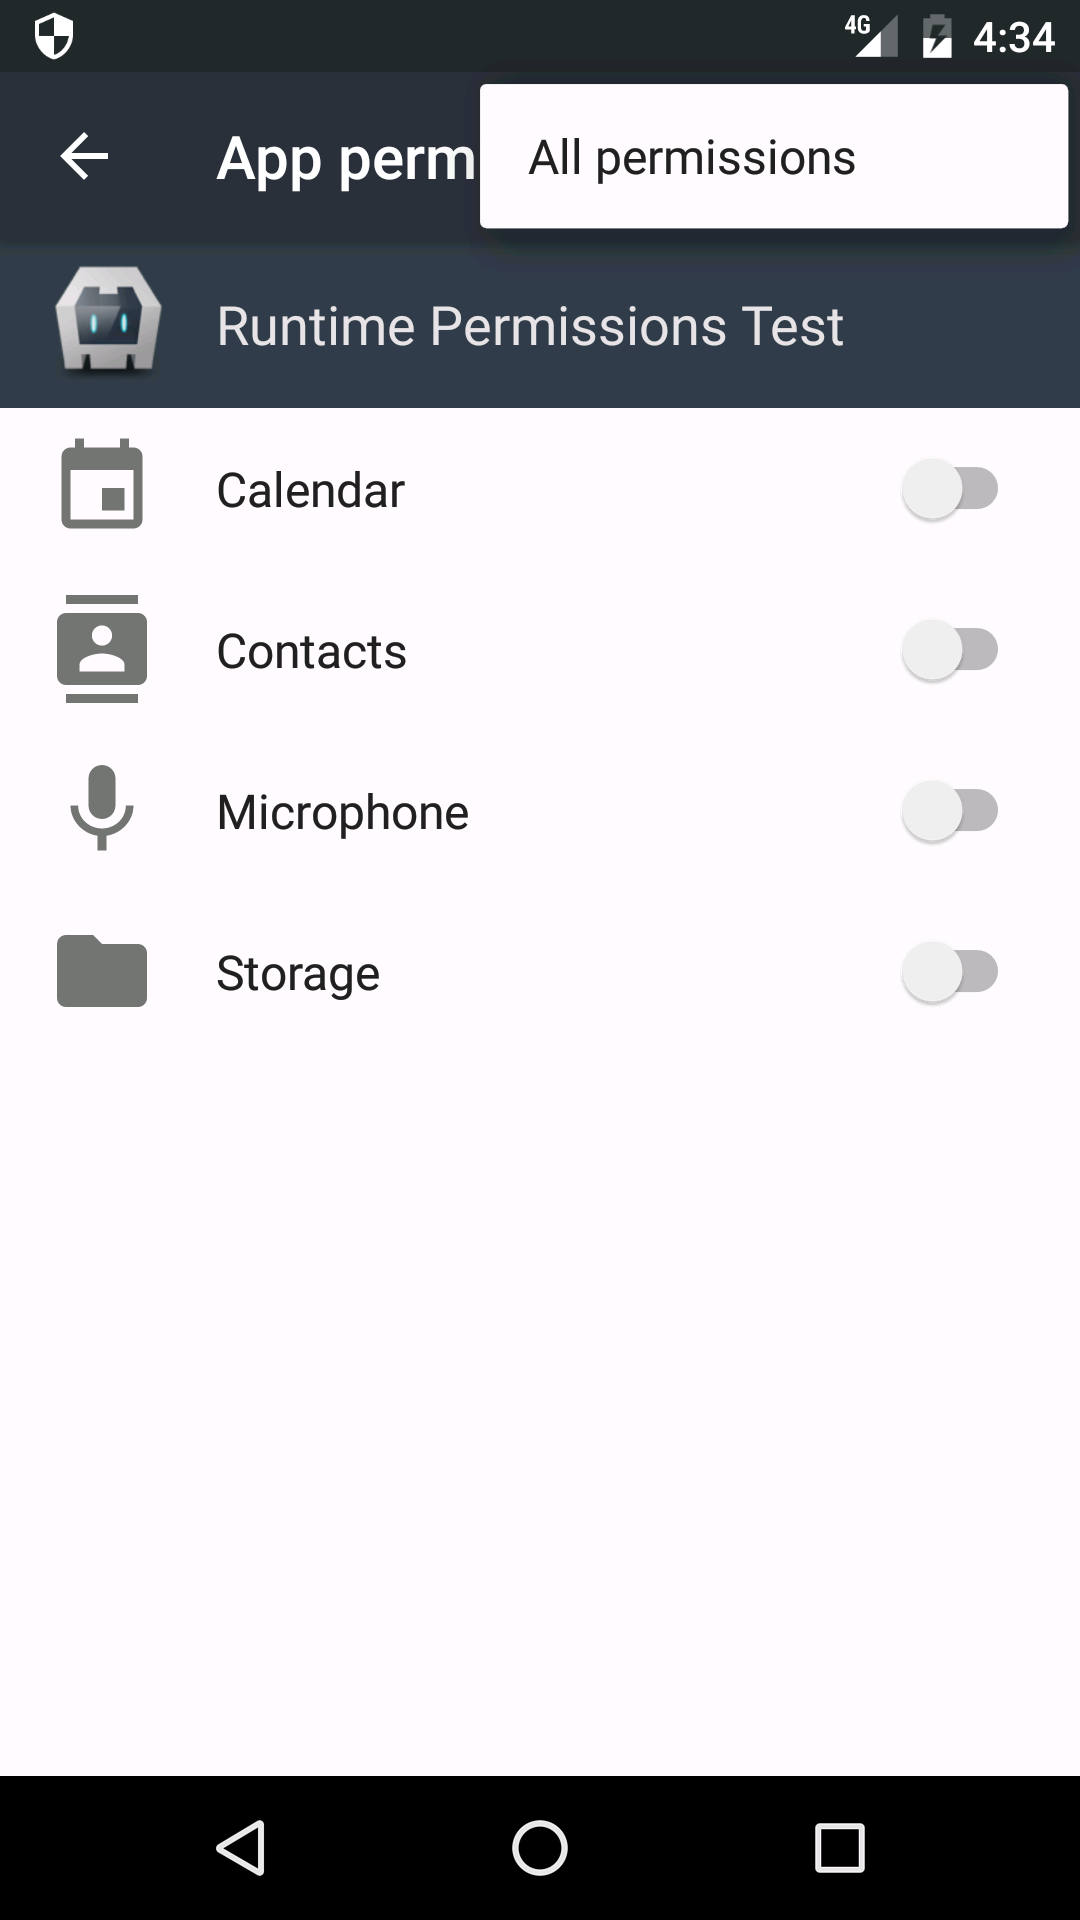
\includegraphics[width=4cm]{chapter5/all_permissions}
		\caption{Si se presiona sobre los tres puntos, se acceden a todos los permisos}
		\label{fig:chapter05:all_permissions}
	\end{subfigure}
	\begin{subfigure}{.32\textwidth}
		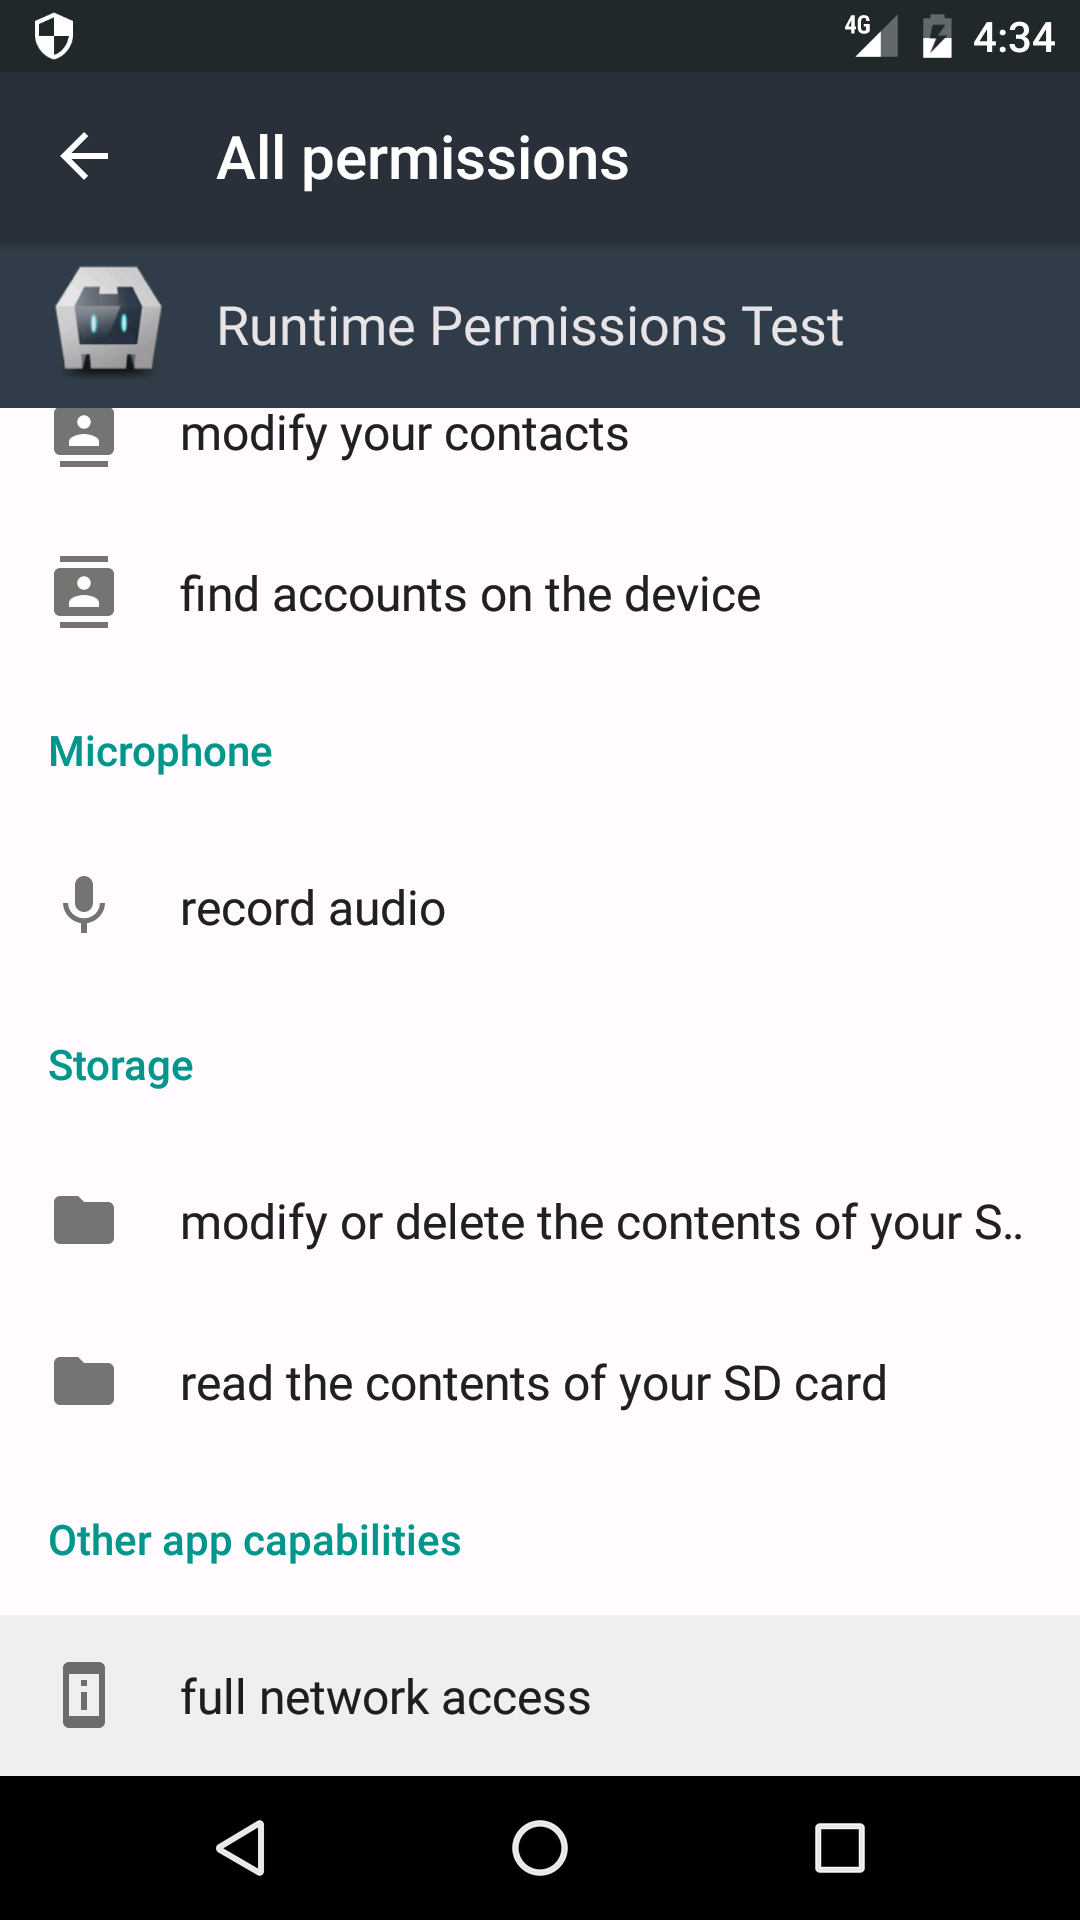
\includegraphics[width=4cm]{chapter5/always_have_internet}
		\caption{\textit{Runtime Permissions Test} tiene todos los permisos $normales$}
		\label{fig:chapter05:always_have_internet}
	\end{subfigure}
	\caption{\textit{Android App Permissions, API\textgreater 23}}
	\label{fig:chapter05:android_permissions}
\end{figure}\\
Sin embargo, si se muestran todos los permisos de la aplicación, notará que se tienen todos los permisos $normales$ que requiera. Por ejemplo, en la Figura \ref{fig:chapter05:always_have_internet} se observa que tenemos permiso de acceso a internet.